\section{Descripcion de los subsistemas del sistema a desarrollar} 
\begin{textoazul}
Incluir si es necesario la descomposición del sistema en subsistemas. Se incluirá un diagrama de bloques u organigramapor claridad

Esta sección podrá omitirse si el sistema software a desarrollar es lo suficientemente sencillo como para no ser dividido en subsistemas.
\end{textoazul}


 \begin{Artefacto}[H]
 \centering
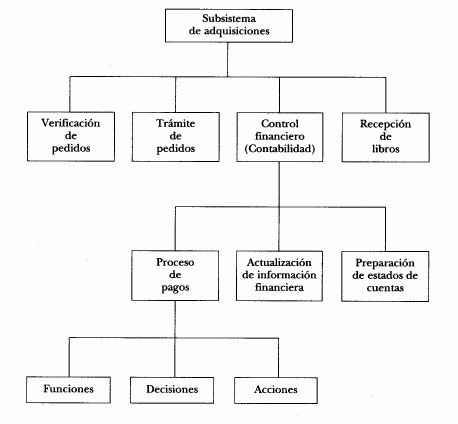
\includegraphics[width=0.8\textwidth]{\fig/organi.jpg}
 \caption{SUB 999	$<nombre descriptivo>$}
 \end{Artefacto}


 \begin{Artefacto}[H]
    \centering
    \begin{tabular}{|p{3cm}|p{10cm}|}
        \hline
         \cellcolor{gray30}  SUB-PRO 999	&  $<nombre descriptivo>$\\ 
%      \cellcolor{gray30}  SUB-PRO 999	& <descriptive name>\\   
        \hline
         \cellcolor{gray30}  [Versión]	&  $<$nº versión$>$($<$fecha de versión$>$)\\   
%      \cellcolor{gray30}  [Version]	&   $<$nº version$>$($<$date$>$)\\   
         \hline
         \cellcolor{gray30}  [Dependencias] &  	\begin{itemize} \item $<objetivos de negocio que comprende>$
\item	$<proceso de negocio con que se relaciona>$ \end{itemize}\\  
%                 \cellcolor{gray30}  [Dependencies] &  	\begin{itemize} \item $<$business processes this actor is involved in$>$
%\item	... \end{itemize}\\            
        \hline
        \cellcolor{gray30} Descripción	& Este subsistema representa a $<descripcion >$  \\
%      \cellcolor{gray30}   Description	& descrip\\   
        \hline
         \cellcolor{gray30}[Importancia]	& $<importancia del proceso de negocio para el cliente>$  \\
%      \cellcolor{gray30}   [Importance] 	& descrip\\   
        \hline
         \cellcolor{gray30}  [Prioridad] &  	$<prioridad para la direccion del proyecto>$\\
%                 \cellcolor{gray30}  [Priority] &   	\\  
         \hline
         \cellcolor{gray30}  Comentarios	&$<comentarios adicionales >$\\   
%         \cellcolor{gray30} Comments	&$<$additional comments$>$
        \hline
  
    \end{tabular}
\caption{SUB-999	$<nombre descriptivo>$ }
%\caption{SUB-999	$<descriptive name>$ }
  \end{Artefacto}



